\section{Pippo Francfrog}\label{pippo-francfrog}
\section{Pippo Francfrog}\label{pippo-francfrog-1}


\begin{figure}
\centering
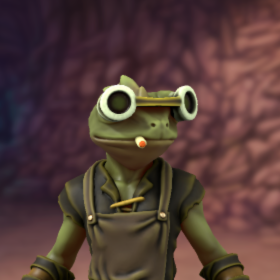
\includegraphics{Pippo_Francfrog-Token.png}
\caption{Pippo Francfrog-Token.png}
\end{figure}

Informazioni Generali

Età:

Anno di nascita:

Paese di nascita:

Razza: Frogfolk

Relazioni:

Alleati:

Nemesi:

Possedimenti importanti:


\subsection{1. Descrizione Generale}\label{descrizione-generale}


\begin{figure}
\centering
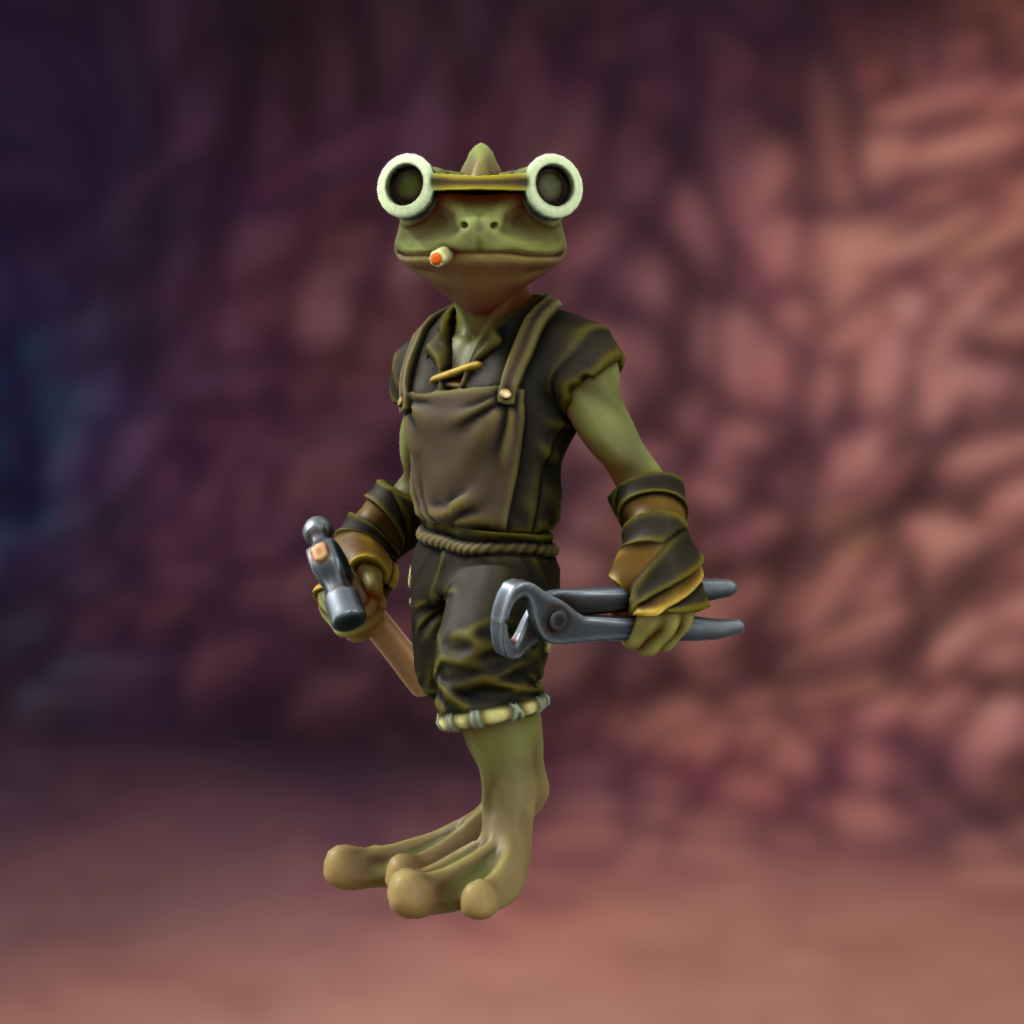
\includegraphics{Pippo_Francfrog-portrait.png}
\caption{Pippo Francfrog-portrait.png}
\end{figure}

Pippo Francfrog incarna l'incantevole fusione di una rana umanoide e la
magia dell'intrattenimento. La sua pelle iridescente rivela radici
anfibie, mentre lo sguardo intelligente brilla di carisma. Con abiti
vivaci e un sorriso contagioso, Pippo attrae l'attenzione ovunque vada.
La sua natura di artista si riflette in ogni gesto, mantenendo viva la
luce del palcoscenico anche mentre esplora nuovi orizzonti.

\begin{quote}
``Torte in faccia!''
\end{quote}

\subsection{2. Biografia}\label{biografia}


\subsubsection{2.1 Infanzia e le Origini
Mistiche}\label{infanzia-e-le-origini-mistiche}

Pippo Francfrog vide la luce grazie a un incantesimo complesso e ardito
lanciato dal mago Lasalmadi Mikebongiorno. La sua creazione era un
tentativo di fondere la magia con il mondo dell'intrattenimento,
producendo così una creatura unica nel suo genere. Sin dalla sua
nascita, Pippo ha portato con sé un legame con la magia che avrebbe
influenzato il corso della sua vita.

\subsubsection{\texorpdfstring{2.2 \textbf{Esordi in ``Il
Bagaglione''}}{2.2 Esordi in ``Il Bagaglione''}}\label{esordi-in-il-bagaglione}

I primi passi di Pippo nel mondo dell'intrattenimento li compì entrando
a far parte dello spettacolo itinerante de ``Il Bagaglione''. Qui, Pippo
fu introdotto all'arte dell'intrattenimento e imparò i segreti
dell'interazione con il pubblico. Le sue performance coinvolgenti e
innovative catturarono l'attenzione di tutti coloro che ebbero la
fortuna di assistere ai suoi numeri.

\subsubsection{\texorpdfstring{2.3 \textbf{Richiamo della Magia e il
Percorso come
Artificiere}}{2.3 Richiamo della Magia e il Percorso come Artificiere}}\label{richiamo-della-magia-e-il-percorso-come-artificiere}

Mentre il suo talento nel campo dell'intrattenimento si faceva sempre
più evidente, la sua connessione con la magia iniziò a emergere in modo
più preponderante. Sentendo il richiamo della magia dentro di sé, Pippo
intraprese un nuovo cammino come artificiere. La sua abilità nel creare
oggetti incantati e invenzioni uniche gli permise di esprimere la sua
creatività in modi mai sperimentati prima.

\subsubsection{\texorpdfstring{2.4 \textbf{Unione Fraterna con Pippo
Baudog}}{2.4 Unione Fraterna con Pippo Baudog}}\label{unione-fraterna-con-pippo-baudog}

Le avventure di Pippo non furono mai solitarie. Insieme a suo fratello
Pippo Baudog, un cane antropomorfo con il medesimo retaggio magico,
intraprese molte imprese. La loro partnership rappresentava l'armoniosa
fusione tra intrattenimento e abilità magica, dimostrando il valore
dell'affetto fraterno nel raggiungimento dei traguardi.

\subsubsection{\texorpdfstring{2.5 \textbf{Eredità e
Impatto}}{2.5 Eredità e Impatto}}\label{eredituxe0-e-impatto}

La vita di Pippo Francfrog è rimasta una testimonianza dell'incrocio tra
il mondo della magia e dell'intrattenimento. La sua biografia incarna la
perseveranza nella ricerca della propria passione, nonostante le diverse
sfaccettature della sua identità. La sua eredità continua a ispirare
coloro che cercano di fondere passioni divergenti, aprendo la strada a
un mondo di meraviglia, sorpresa e collaborazione.

\subsection{3. Carriera}\label{carriera}


La carriera di Pippo Francfrog è stata un connubio straordinario tra
magia e intrattenimento. Dopo esordi di successo con lo spettacolo
itinerante de ``Il Bagaglione'', Pippo ha seguito il richiamo della
magia e si è dedicato all'artigianato magico come artificiere.
Nonostante questo cambiamento di percorso, non ha mai dimenticato le sue
radici da intrattenitore, portando sempre con sé il desiderio di
incantare e stupire il pubblico. Collaborando spesso con suo fratello,
